% Options for packages loaded elsewhere
\PassOptionsToPackage{unicode}{hyperref}
\PassOptionsToPackage{hyphens}{url}
%
\documentclass[
  twocolumn]{article}
\usepackage{amsmath,amssymb}
\usepackage{lmodern}
\usepackage{ifxetex,ifluatex}
\ifnum 0\ifxetex 1\fi\ifluatex 1\fi=0 % if pdftex
  \usepackage[T1]{fontenc}
  \usepackage[utf8]{inputenc}
  \usepackage{textcomp} % provide euro and other symbols
\else % if luatex or xetex
  \usepackage{unicode-math}
  \defaultfontfeatures{Scale=MatchLowercase}
  \defaultfontfeatures[\rmfamily]{Ligatures=TeX,Scale=1}
\fi
% Use upquote if available, for straight quotes in verbatim environments
\IfFileExists{upquote.sty}{\usepackage{upquote}}{}
\IfFileExists{microtype.sty}{% use microtype if available
  \usepackage[]{microtype}
  \UseMicrotypeSet[protrusion]{basicmath} % disable protrusion for tt fonts
}{}
\makeatletter
\@ifundefined{KOMAClassName}{% if non-KOMA class
  \IfFileExists{parskip.sty}{%
    \usepackage{parskip}
  }{% else
    \setlength{\parindent}{0pt}
    \setlength{\parskip}{6pt plus 2pt minus 1pt}}
}{% if KOMA class
  \KOMAoptions{parskip=half}}
\makeatother
\usepackage{xcolor}
\IfFileExists{xurl.sty}{\usepackage{xurl}}{} % add URL line breaks if available
\IfFileExists{bookmark.sty}{\usepackage{bookmark}}{\usepackage{hyperref}}
\hypersetup{
  pdftitle={CSC 8634 - Cloud Computing},
  pdfauthor={Marc Birkett},
  hidelinks,
  pdfcreator={LaTeX via pandoc}}
\urlstyle{same} % disable monospaced font for URLs
\usepackage[margin=1in]{geometry}
\usepackage{color}
\usepackage{fancyvrb}
\newcommand{\VerbBar}{|}
\newcommand{\VERB}{\Verb[commandchars=\\\{\}]}
\DefineVerbatimEnvironment{Highlighting}{Verbatim}{commandchars=\\\{\}}
% Add ',fontsize=\small' for more characters per line
\usepackage{framed}
\definecolor{shadecolor}{RGB}{248,248,248}
\newenvironment{Shaded}{\begin{snugshade}}{\end{snugshade}}
\newcommand{\AlertTok}[1]{\textcolor[rgb]{0.94,0.16,0.16}{#1}}
\newcommand{\AnnotationTok}[1]{\textcolor[rgb]{0.56,0.35,0.01}{\textbf{\textit{#1}}}}
\newcommand{\AttributeTok}[1]{\textcolor[rgb]{0.77,0.63,0.00}{#1}}
\newcommand{\BaseNTok}[1]{\textcolor[rgb]{0.00,0.00,0.81}{#1}}
\newcommand{\BuiltInTok}[1]{#1}
\newcommand{\CharTok}[1]{\textcolor[rgb]{0.31,0.60,0.02}{#1}}
\newcommand{\CommentTok}[1]{\textcolor[rgb]{0.56,0.35,0.01}{\textit{#1}}}
\newcommand{\CommentVarTok}[1]{\textcolor[rgb]{0.56,0.35,0.01}{\textbf{\textit{#1}}}}
\newcommand{\ConstantTok}[1]{\textcolor[rgb]{0.00,0.00,0.00}{#1}}
\newcommand{\ControlFlowTok}[1]{\textcolor[rgb]{0.13,0.29,0.53}{\textbf{#1}}}
\newcommand{\DataTypeTok}[1]{\textcolor[rgb]{0.13,0.29,0.53}{#1}}
\newcommand{\DecValTok}[1]{\textcolor[rgb]{0.00,0.00,0.81}{#1}}
\newcommand{\DocumentationTok}[1]{\textcolor[rgb]{0.56,0.35,0.01}{\textbf{\textit{#1}}}}
\newcommand{\ErrorTok}[1]{\textcolor[rgb]{0.64,0.00,0.00}{\textbf{#1}}}
\newcommand{\ExtensionTok}[1]{#1}
\newcommand{\FloatTok}[1]{\textcolor[rgb]{0.00,0.00,0.81}{#1}}
\newcommand{\FunctionTok}[1]{\textcolor[rgb]{0.00,0.00,0.00}{#1}}
\newcommand{\ImportTok}[1]{#1}
\newcommand{\InformationTok}[1]{\textcolor[rgb]{0.56,0.35,0.01}{\textbf{\textit{#1}}}}
\newcommand{\KeywordTok}[1]{\textcolor[rgb]{0.13,0.29,0.53}{\textbf{#1}}}
\newcommand{\NormalTok}[1]{#1}
\newcommand{\OperatorTok}[1]{\textcolor[rgb]{0.81,0.36,0.00}{\textbf{#1}}}
\newcommand{\OtherTok}[1]{\textcolor[rgb]{0.56,0.35,0.01}{#1}}
\newcommand{\PreprocessorTok}[1]{\textcolor[rgb]{0.56,0.35,0.01}{\textit{#1}}}
\newcommand{\RegionMarkerTok}[1]{#1}
\newcommand{\SpecialCharTok}[1]{\textcolor[rgb]{0.00,0.00,0.00}{#1}}
\newcommand{\SpecialStringTok}[1]{\textcolor[rgb]{0.31,0.60,0.02}{#1}}
\newcommand{\StringTok}[1]{\textcolor[rgb]{0.31,0.60,0.02}{#1}}
\newcommand{\VariableTok}[1]{\textcolor[rgb]{0.00,0.00,0.00}{#1}}
\newcommand{\VerbatimStringTok}[1]{\textcolor[rgb]{0.31,0.60,0.02}{#1}}
\newcommand{\WarningTok}[1]{\textcolor[rgb]{0.56,0.35,0.01}{\textbf{\textit{#1}}}}
\usepackage{graphicx}
\makeatletter
\def\maxwidth{\ifdim\Gin@nat@width>\linewidth\linewidth\else\Gin@nat@width\fi}
\def\maxheight{\ifdim\Gin@nat@height>\textheight\textheight\else\Gin@nat@height\fi}
\makeatother
% Scale images if necessary, so that they will not overflow the page
% margins by default, and it is still possible to overwrite the defaults
% using explicit options in \includegraphics[width, height, ...]{}
\setkeys{Gin}{width=\maxwidth,height=\maxheight,keepaspectratio}
% Set default figure placement to htbp
\makeatletter
\def\fps@figure{htbp}
\makeatother
\setlength{\emergencystretch}{3em} % prevent overfull lines
\providecommand{\tightlist}{%
  \setlength{\itemsep}{0pt}\setlength{\parskip}{0pt}}
\setcounter{secnumdepth}{-\maxdimen} % remove section numbering
\ifluatex
  \usepackage{selnolig}  % disable illegal ligatures
\fi

\title{CSC 8634 - Cloud Computing}
\author{Marc Birkett}
\date{17/12/2021}

\begin{document}
\maketitle

\hypertarget{introduction}{%
\subsection{Introduction}\label{introduction}}

This project is an exploratory data analysis (EDA) project into a
multiple GPU node map rendering system. To bring structure to this
project the CRISP-DM methodology will be followed as ``it is soundly
based on the practical, real-world experience of how people conduct data
mining projects.'' (Chapman et al, 2000). To aid organisation and
repeatability of the project various packages from the Tidyverse will be
used, particularly ReadR, DPlyr, GGPlot2 and ProjectTemplate. The
methodology splits a data mining project into 5 stages which will
provide structure to this document, these are Business Understanding,
Data Understanding, Data Preparation, Modelling and Evaluation.

\hypertarget{business-understanding}{%
\subsection{Business Understanding}\label{business-understanding}}

\textcolor{red}{(Business objectives, assess situation, goals, project plan)}

\textcolor{red}{What is the need for the project? - Justify your choice of response (i.e. the nature of, and your plan for, your project). To give strength to your argument, you should reference to practice elsewhere (e.g. in academic literature, or industry practices.}

Cloud computing has became more commonly used throughout all sectors in
the UK since 2000. Multiple providers such as Amazon and Microsoft are
now in a marketplace which seeks to offer externally hosted solutions on
a Software as a Service (SaaS) basis, along with infrastructure and
platforms to provide eslastic, scalable solutions to business need.
Along with this there is an opportunity to bring rigour to the
measurement and evaluation of cloud computing approaches. A Research and
literature review into the subject was carried out via Google Scholar.
The terms ``statistical rigour, reproducible data analyses, performance
evaluation in computer science'' produced 7.94 million results. The
addition of keywords including ``cloud computing'' and ``supercomputer''
brought this down to 44,600 records. A selection of highly referenced
documents was reviewed.

Hoefler, Torsten and Belli (2015) state that the ``measuring and
reporting performance of parallel computers constitute the basis of
scientific advancement of high performance computing \ldots{} and that
the state of practice is lacking''. Vitek and Kalibera, 2011, lamented
``unrepeatable results, unreproduced results, lack of benchmarks, lack
of experimental methodology'', and, Papadopoulos et al, 2018, ``although
these important principles are simple and basic, the cloud community is
yet to adopt them broadly to deliver sound measurement of cloud
environments.''. Given this lack of rigour, this paper will be
approached as a exploratory data analysis project.

\hypertarget{problem-area}{%
\subsubsection{Problem Area}\label{problem-area}}

This paper conducts a performance evaluation of terapixel rendering in
cloud super computing. The solution was rendering using an
Infrastructure as a Service (IaaS) cloud environment and up to 1024
graphical process unit (GPU) nodes which was used to compute a realistic
visualisation of Newcastle Upon Tyne and its environmental data as
captured by the Newcastle Urban Observatory. The data was subsequently
provided for analysis via comma separated value files. There will also
subsequently be a dashboard created to allow investigation of the data
set.

The completion of this paper will contribute to the some of knowledge
regarding the measurement and assessment of metrics on cloud based
supercomputers.

\hypertarget{current-solution}{%
\subsubsection{Current Solution}\label{current-solution}}

The project currently demonstrated that it ``is feasible to produce a
high quality terapixel visualization using a path tracing renderer in
under a day using public IaaS cloud GPU nodes. Once generated the
terapixel image supports interactive browsing of the city and its data
at a range of sensing scales from the whole city to a single desk in a
room'' (Forshaw, 2021). However, there has been no analysis of the
metrics produced by the system regarding performance.

\hypertarget{objectives}{%
\subsubsection{Objectives}\label{objectives}}

Various examples of data we can investigate through an EDA process have
been provided with the dataset, which are outlined here:

\begin{itemize}
\tightlist
\item
  Which event types dominate task runtimes?
\item
  What is the interplay between GPU temperature and performance?
\item
  What is the interplay between increased power draw and render time?
\item
  Can we quantify the variation in computation requirements for
  particular tiles?
\item
  Can we identify particular GPU cards (based on their serial numbers)
  whose performance differs to other cards? (i.e.~perpetually slow
  cards).
\item
  What can we learn about the efficiency of the task scheduling process?
\end{itemize}

I am particularly interested in the differing performance of various GPU
cards in use. This work will be applicable to the investigation of other
hardware within the use of the cloud and could be applied to my day to
day work.

\hypertarget{success-criteria-and-project-plan}{%
\subsubsection{Success criteria and Project
Plan}\label{success-criteria-and-project-plan}}

The data provided includes the complete cycle of the rendering of each
graphic, along with the grid, in X and Y co-ordinates for each graphic
and the granularity of the zoom. The success of this project will be
identifying low performing GPU cards based on their render time. The
data provided will be investigated to identify the performance of each
card. The wider dataset will also then be investigated for mitigating
factors such as load, through the potential complexity of the graphic
being rendered and the point in the render process which takes the most
time.

\hypertarget{data-understanding}{%
\subsection{Data Understanding}\label{data-understanding}}

\textcolor{red}{(collect initial data, describe, explore, data quality)}
\textcolor{red}{What, concisely, did you do?} A quick review of the
provided data was completed which identified that the Application
Checkpoint and GPU data could be used to examine performance of each
card. The data was loaded via ProjectTemplate into R studio and
subsequently investigated through examining counts, ``Quartile
Quartile'' plots, and the creation of a gpuStats dataset to create a
boxplot of mean and standard deviation on performance statistics.

To begin to identify the execution time, the Application Checkpoint data
was investigated, this contains time stamps for each step of the image
render process. There are 5 event types each with a start and stop event
recorded. These are Total Render - the complete render event, which is
made up of 4 events which are, in order, Render, Saving Config, Tiling,
Uploading. Initial investigation will cover the total render time, which
will indicate the performance of the GPU, should we get that far we can
look into the time of each stage of the render.

\begin{figure}
\includegraphics[width=1\linewidth]{report_files/figure-latex/hostsCount-1} \caption{Azure Hosts use during Render}\label{fig:hostsCount}
\end{figure}

In the absence of any continuous data in this table basic data quality
checks were carried out, this identified the following:

\begin{itemize}
\tightlist
\item
  All of the START events have an associated STOP event, as there are
  the same number of both.
\item
  All TOTAL RENDER events have a complete set of child events.
\item
  Most host machines were used between 600 and 700 times during the
  course of the data, up to 670 times at the third quartile. However,
  there were 4 host machines that were used in 1240 and 1220 runs
  respectively as shown in Figure 1.
\item
  There are some tasks which were ran twice, hence having 20 instances
  of jobId / taskId pairs in the dataset.
\end{itemize}

Initial investigation of the GPU data indicates that the Hostname can be
used to relate to the GPU on the host, so the 4 spikes of host use may
have implications for that. Some work around the timestamp of each start
and stop event during the data preparation phase will give us the total
and interim render times in seconds. The GPU data gives is statistics
regarding the state of each GPU with a timestamp and data covering
Temperature, Power Draw, Utilised Percentage and Memory Utilised
Percentage. Through the use of a set of Quantile Quantile graph is can
be seen that this data is normalised and therefore we will use the
arithmetic mean as the average, and standard deviation to express the
variance. These can be seen in figure 2 below, it shows us that we have
a complete data set to work with and that the variance for all variables
except temperature is large, which is to be expected as this is the
difference between the GPU being in use, or not. This variance will be
used along with the execution time identified above to indicate poor
performing GPU's. We have also established that we have a complete
dataset in GPU, n=1543681.

\begin{verbatim}
## geom_path: Each group consists of only one observation. Do you need to adjust
## the group aesthetic?
\end{verbatim}

\begin{figure}
\includegraphics[width=1\linewidth]{report_files/figure-latex/gpuStats-1} \caption{GPU Continuous Variable Stats}\label{fig:gpuStats}
\end{figure}

From this investigation phase it is my intention to pull together a
complete dataset to allow comparison of execution times and GPU
performance statistics.

\hypertarget{data-preparation}{%
\subsection{Data Preparation}\label{data-preparation}}

\textcolor{red}{(select, clean, construct, integrate, format)}
\textcolor{red}{What, concisely, did you do?} To identify the lowest
performing GPU cards some feature engineering was carried on the
application checkpoint dataset. The TotalRenderTime measure was
identified as a measure of execution time, so a dataset was created
showing the the hostname, start and end time of the task and total
execution time by casting to date and then subracting the end time from
the start time. An examination of this dataset gives a mean render time
of 42.61 second and a standard deviation of 6.5 seconds. The
distribution shown in Figure 3 with the mean and the upper and lower
quartiles a 1 standard deviation. It can be clearly seen that there is a
tail on the execution times from the upper quartile at 49.1 seconds to a
max of 93.6 seconds.

```\{ r RenderTimeDistribution, out.width=``100\%'',
fig.cap=``Distribution of Mean Total Render Time''\}

\#plot the distribution ggplot(df.execution, aes(x=totalRenderTime)) +
geom\_histogram(aes(y=..density..), \# Histogram with density instead of
count on y-axis binwidth=1, colour=``black'', fill=``white'') +
geom\_density(alpha=.2, fill=``\#FF6666'') + \# Overlay with transparent
density plot geom\_vline(aes(xintercept=mean(totalRenderTime, na.rm=T)),
\# Ignore NA values for mean color=``red'', linetype=``solid'', size=1)
+ geom\_vline(aes(xintercept=mean(totalRenderTime + renderTimeSd,
na.rm=T)), \# Ignore NA values for upper sd color=``red'',
linetype=``dashed'', size=1) +
geom\_vline(aes(xintercept=mean(totalRenderTime - renderTimeSd,
na.rm=T)), \# Ignore NA values for lowersd color=``red'',
linetype=``dashed'', size=1) + labs(title=``Distribution of Total Render
Time in 1 Second Bins'', y=``Density'', x=``Render Time in Seconds'') +
theme\_bw() + scale\_fill\_brewer(palette=``PuBu'')

\begin{verbatim}
Those hosts above the upper quartile were taken as the dataset of long running hosts. The number of occurance of each host within the upper quartile was then counted which have a mean of 8.0 times and a standard deviation of 6.01. Therefore the upper quartile of this was also taken, so any host which occured in the upper quartile of long running hosts more than 14.02 times was regarded as the final dataset for investigation. This yielded a dataset of 154 records, which when joined back to the execution time table gives 9563 tasks on the longest running hosts, complete with total render time. 

This is still a lot of records to investigate.

In an effort to reduce the volume of records the number of tasks in this long running set was investigated, by the maximum recurrence of a taskId was 2, so this was ignored. I then attempted to take the upper quartile of the long running hosts which results in 843 records to work with, and attempt to relate the GPU dataset to allow identification of the specific GPU being used in the long running tasks.

Upon investigation of the GPU dataset, it was found that virtually all host names were in the long running hosts top percentiles, and multiple GPU cards were assigned to each hostname and were "active" between the start and end times. It was assumed that a task to render a certain plot was split across all GPU on the host, so the render time was appended to the row identifying each GPU. This gives us the following dataset to work with:

* Timestamp
* Hostname
* GPU Serial
* GPU UUID
* Power Draw (Watts)
* GPU Temp (C)
* GPU Util Percent
* GPU Mem Util Percent
* Total Render Time

with a total of 23,754 records to investigate.

## Modelling 
\textcolor{red}{(technique, test design, build, assess) R-Shiny}
\textcolor{red}{What, concisely, did you do?}
For the intial investigation the dataset above was slimmed down to just the hostname, gpu serial name and hosts render time, this dropped out 'duplicate' records which were tenths of a second different. This dataset was than investigated for commonly occurring hosts and GPU. As per the figures below it can be seen that there are multiple occurances of certain hosts and GPU in the longest running tasks data set.

```{ r countOfHosts, out.width="100%", fig.cap="Hostname occurence in longest running tasks."}
#plot the occurrence of hosts
ggplot(data=df.longestGPUSlim %>% count(hostname), aes(as.character(hostname), y=n, group=1)) +
  geom_line() +
  labs(title="Number of occurances of hostname in the top percentile longest running tasks", 
       y="Count", x = "Hostname") 
  theme_bw() + 
  scale_fill_brewer(palette="PuBu") +
  theme(axis.text.x = element_text(angle = 90))
\end{verbatim}

\texttt{\{\ r\ countOfGPU,\ out.width="100\%",\ fig.cap="GPU\ Serial\ occurence\ in\ longest\ running\ tasks."\}\ \#plot\ the\ occurrence\ of\ gpus\ ggplot(data=df.longestGPUSlim\ \%\textgreater{}\%\ count(gpuSerial),\ aes(as.character(gpuSerial),\ y=n,\ group=1))\ +\ \ \ geom\_line()\ +\ \ \ labs(title="Number\ of\ occurances\ of\ GPU\ in\ the\ top\ percentile\ longest\ running\ tasks",\ \ \ \ \ \ \ \ \ y="Count",\ x\ =\ "GPU\ Serial")\ +\ \ \ theme\_bw()\ +\ \ \ \ scale\_fill\_brewer(palette="PuBu")\ +\ \ \ theme(axis.text.x\ =\ element\_text(angle\ =\ 90))}

Further investigation of the dataset allows us to glean the hostname of
the longest running task, the time and the GPU, which answers the
question of ``which is the worst performing GPU'', in a general way.

\begin{Shaded}
\begin{Highlighting}[]
\NormalTok{longestHostname }\OtherTok{=}\NormalTok{ df.jobsbyrendertime[}\DecValTok{1}\NormalTok{,}\DecValTok{1}\NormalTok{]}
\NormalTok{longestGPUSerial }\OtherTok{=}\NormalTok{ df.jobsbyrendertime[}\DecValTok{1}\NormalTok{,}\DecValTok{2}\NormalTok{]}
\NormalTok{longestHostTime }\OtherTok{=}\NormalTok{ df.jobsbyrendertime[}\DecValTok{1}\NormalTok{,}\DecValTok{3}\NormalTok{]}
\end{Highlighting}
\end{Shaded}

However, this doesn't allow us to properly investigate that dataset, the
raw data regarding execution time means nothing without knowing the work
that was carried out. For example, potentially consistently rendering
the same grid on the same host, where that grid is particularly complex
or has a lot of items to render, would result in a long render time for
that host. However, it does not particularly mean that host is
underperforming. We should also be able to investigate multiple GPU on
multiple hosts. I am also not convinced that showing one GPU per
hostname represents the dataset.

Subsequently, after re-iteration through the understanding and
preparation tasks, the taskId and jobId was added to the dataset for
investigation, to allow association with the grid being rendered. I will
also output an ungrouped dataset for the creation of a dashboard. An
investigation of render time by the X, Y grid references as per figure
below does not seem to indicate any consistency in certain refs being
long render times. We should look at other potential issues.

\texttt{\{\ r\ RenderByRef,\ out.width="100\%",\ fig.cap="Longest\ running\ task\ hostname,\ serial\ and\ time."\}\ ggplot(df.longestGPUGrid,\ aes(XY,\ hostLongestRenderTime))\ +\ \ \ \ geom\_point()\ +\ \ \ labs(title="Render\ Time\ by\ Grid\ Reference",\ y="Render\ Time",\ x\ =\ "Grid\ Reference(XY)")\ +\ \ \ theme\_bw()\ +\ \ \ \ scale\_fill\_brewer(palette="PuBu")\ +\ \ \ theme(axis.text.x\ =\ element\_text(angle\ =\ 90))}

A similar investigation into the metrics provided for each GPU also
indicates no relationship. In fact percentage utilisation and memory
utilisation are null. There is no obvious relationship for Temperature
or Power Draw.

```\{ r RenderByMetrics, out.width=``100\%'', fig.cap=``Render Time vs
GPU metrics.''\} \#render time vs cpu state powerDraw
ggplot(df.longestGPUGrid, aes(powerDrawWatt , hostLongestRenderTime)) +
geom\_point() + labs(title=``Render Time by GPU Power Draw'', y=``Render
Time'', x = ``Power Draw in Watts'') + theme\_bw() +
scale\_fill\_brewer(palette=``PuBu'') + theme(axis.text.x =
element\_text(angle = 90))

\#render time vs cpu state temp ggplot(df.longestGPUGrid, aes(gpuTempC,
hostLongestRenderTime)) + geom\_point() + labs(title=``Render Time by
GPU Temp'', y=``Render Time'', x = ``Temp in C'') + theme\_bw() +
scale\_fill\_brewer(palette=``PuBu'') + theme(axis.text.x =
element\_text(angle = 90)) ``` In an effort to find some meaningful data
a dashboard was created. Before creating the dashboard, the dataset was
investigated for the relationships within the dataset, the following was
concluded:

\begin{itemize}
\tightlist
\item
  There are three jobIds which indicate the level of the grid being
  rendered. The busiest level is level 12.
\item
  Each job has many tasks, which pertain to each job square being
  rendered.
\item
  Each task has one grid square.
\item
  One task is executed on one host machine.
\item
  One task is executed on one GPU care on one host machine.
\item
  Each GPU is in the dataset for many seconds of the longest render
  time.
\end{itemize}

This it was concluded if we can select the level of the render to be
investigated, then we can show the grids being rendered, the the 1:1
hosts and GPU being used to render it. Upon creating the dashboard the
level can be selected, the render times of each grid x,y reference and a
list of Host and GPU ordered by render time with the longest to the top.
This answers the question with the output in the figure below.

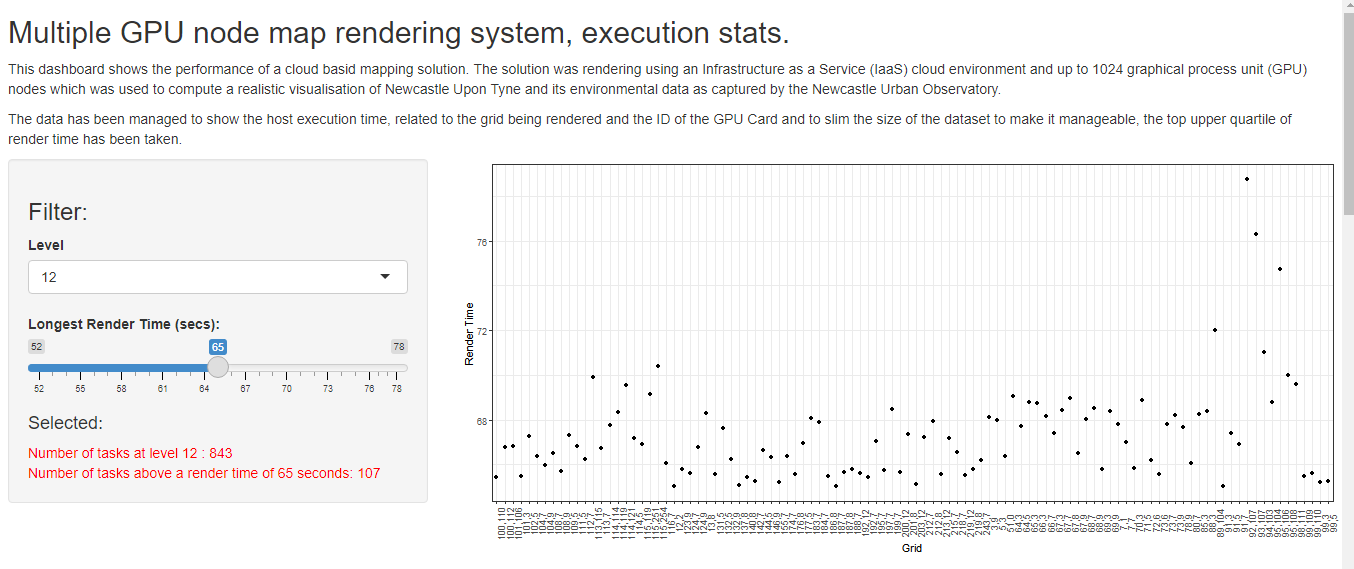
\includegraphics{/graphs/ExecutionTimesGraph.png}
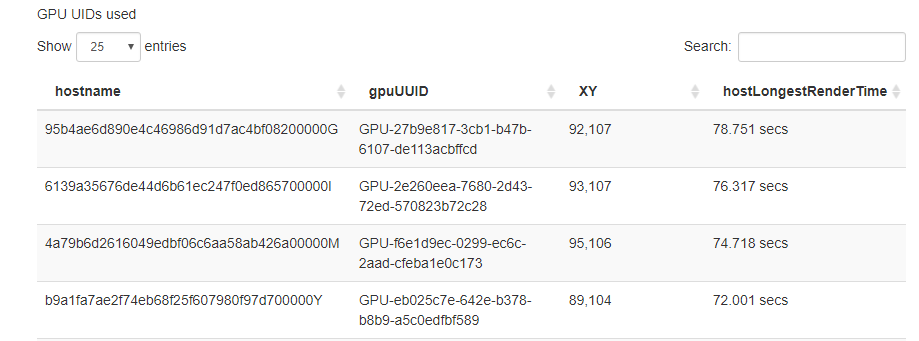
\includegraphics{/graphs/LongestRenderTimes.png}

It can clearly be seen that the longest execution time is host
`95b4ae6d890e4c46986d91d7ac4bf08200000G', GPU ID
`GPU-27b9e817-3cb1-b47b-6107-de113acbffcd' rendering grid `92,107'.

\hypertarget{evaluation}{%
\subsection{Evaluation}\label{evaluation}}

\textcolor{red}{(evaluate, review, next steps)}
\textcolor{red}{How successful has it been? Provide evidence, using appropriate evaluation methodologies, and comment on the strengths/weaknesses of your evidence in answering this question. What are the future implications for work in this area? If applicable, which areas of extension work are now possible due to the foundational work you have performed in this project?}

To result in a dataset which my laptop was capable of processing, we
have in effect taken the upper quartile of response times, followed by
taking a second upper quartile. While taking all of the responses which
are above a quartile away from the mean is a sound method of identifying
the longest running records I am not entirely comfortable with taking
another subset merely to fit with the performance limitations of this
machine.

Also, I would have expected multiple GPU ID cards to be found slowly
performing on a host on any given task, but that isn't what the data has
provided. I am not entirely sure that taking the cards which are showing
some activity within the overall task start and finish time, although on
the correct host, have identified the complete set of cards. I am hoping
that because of the way I have limited the dataset this has
coincidentally produced a 1 to 1 dataset between host and GPU. Given
more time and more processing power I would have liked to have
investigated the dataset further, and potentially looked to export the
data via CSV to a specialist visualisation tool such as PowerBI. I found
the time investment in Shiny to be useful without being massively
productive.

\hypertarget{references}{%
\subsection{References}\label{references}}

Alessandro V. Papadopoulos, Senior Member, IEEE, Laurens Versluis,
Member, IEEE, Andre Bauer, Nikolas Herbst, Member, IEEE, Joakim von
Kistowski, Member, IEEE, Ahmed Ali-Eldin, Cristina L. Abad, Member,
IEEE, Jose Nelson Amaral, Senior Member, IEEE, Petr Tuma, Member, IEEE,
and Alexandru Iosup, Member, IEEE, 2018, Methodological Principles for
Reproducible Performance Evaluation in Cloud Computing,
\url{https://drive.google.com/file/d/151guslA9SYV-8BJNMXa1udvMrF4jn2ae/view}
Accessed: 21/12/2021

Forshaw, Matt, 2021, Performance evaluation of Terapixel rendering in
Cloud (Super)computing
{[}\url{https://github.com/NewcastleDataScience/StudentProjects202122/blob/master/TeraScope/Summary.md\#background}{]}
(\url{https://github.com/NewcastleDataScience/StudentProjects202122/blob/master/TeraScope/Summary.md\#background})
Accessed: 21/12/2021

Hoefler, Torsten, and Roberto Belli, 2015, ``Scientific benchmarking of
parallel computing systems: twelve ways to tell the masses when
reporting performance results.'' In Proceedings of the international
conference for high performance computing, networking, storage and
analysis, p.~73. ACM, 2015.

Jan Vitek, Tomas Kalibera, 2011, Repeatability, Reproducibility and
Rigor in Systems Research
\url{https://www.cs.kent.ac.uk/pubs/2011/3174/content.pdf} Accessed:
21/12/2021

Pete Chapman (NCR), Julian Clinton (SPSS), Randy Kerber (NCR), Thomas
Khabaza (SPSS), Thomas Reinartz (DaimlerChrysler), Colin Shearer (SPSS)
and Rüdiger Wirth (DaimlerChrysler), 2000, CRISP-DM Step-by-step data
mining guide

\end{document}
